% Options for packages loaded elsewhere
\PassOptionsToPackage{unicode}{hyperref}
\PassOptionsToPackage{hyphens}{url}
%
\documentclass[
]{article}
\title{Projet LSTAT2110(A) -- Analyse de données}
\author{PETIT Romain \& VAN GEERSDAELE Arthur, 4827-1700 \& 3004-1700,
GBIO2M}
\date{}

\usepackage{amsmath,amssymb}
\usepackage{lmodern}
\usepackage{iftex}
\ifPDFTeX
  \usepackage[T1]{fontenc}
  \usepackage[utf8]{inputenc}
  \usepackage{textcomp} % provide euro and other symbols
\else % if luatex or xetex
  \usepackage{unicode-math}
  \defaultfontfeatures{Scale=MatchLowercase}
  \defaultfontfeatures[\rmfamily]{Ligatures=TeX,Scale=1}
\fi
% Use upquote if available, for straight quotes in verbatim environments
\IfFileExists{upquote.sty}{\usepackage{upquote}}{}
\IfFileExists{microtype.sty}{% use microtype if available
  \usepackage[]{microtype}
  \UseMicrotypeSet[protrusion]{basicmath} % disable protrusion for tt fonts
}{}
\makeatletter
\@ifundefined{KOMAClassName}{% if non-KOMA class
  \IfFileExists{parskip.sty}{%
    \usepackage{parskip}
  }{% else
    \setlength{\parindent}{0pt}
    \setlength{\parskip}{6pt plus 2pt minus 1pt}}
}{% if KOMA class
  \KOMAoptions{parskip=half}}
\makeatother
\usepackage{xcolor}
\IfFileExists{xurl.sty}{\usepackage{xurl}}{} % add URL line breaks if available
\IfFileExists{bookmark.sty}{\usepackage{bookmark}}{\usepackage{hyperref}}
\hypersetup{
  pdftitle={Projet LSTAT2110(A) -- Analyse de données},
  pdfauthor={PETIT Romain \& VAN GEERSDAELE Arthur, 4827-1700 \& 3004-1700, GBIO2M},
  hidelinks,
  pdfcreator={LaTeX via pandoc}}
\urlstyle{same} % disable monospaced font for URLs
\usepackage[margin=1in]{geometry}
\usepackage{color}
\usepackage{fancyvrb}
\newcommand{\VerbBar}{|}
\newcommand{\VERB}{\Verb[commandchars=\\\{\}]}
\DefineVerbatimEnvironment{Highlighting}{Verbatim}{commandchars=\\\{\}}
% Add ',fontsize=\small' for more characters per line
\usepackage{framed}
\definecolor{shadecolor}{RGB}{248,248,248}
\newenvironment{Shaded}{\begin{snugshade}}{\end{snugshade}}
\newcommand{\AlertTok}[1]{\textcolor[rgb]{0.94,0.16,0.16}{#1}}
\newcommand{\AnnotationTok}[1]{\textcolor[rgb]{0.56,0.35,0.01}{\textbf{\textit{#1}}}}
\newcommand{\AttributeTok}[1]{\textcolor[rgb]{0.77,0.63,0.00}{#1}}
\newcommand{\BaseNTok}[1]{\textcolor[rgb]{0.00,0.00,0.81}{#1}}
\newcommand{\BuiltInTok}[1]{#1}
\newcommand{\CharTok}[1]{\textcolor[rgb]{0.31,0.60,0.02}{#1}}
\newcommand{\CommentTok}[1]{\textcolor[rgb]{0.56,0.35,0.01}{\textit{#1}}}
\newcommand{\CommentVarTok}[1]{\textcolor[rgb]{0.56,0.35,0.01}{\textbf{\textit{#1}}}}
\newcommand{\ConstantTok}[1]{\textcolor[rgb]{0.00,0.00,0.00}{#1}}
\newcommand{\ControlFlowTok}[1]{\textcolor[rgb]{0.13,0.29,0.53}{\textbf{#1}}}
\newcommand{\DataTypeTok}[1]{\textcolor[rgb]{0.13,0.29,0.53}{#1}}
\newcommand{\DecValTok}[1]{\textcolor[rgb]{0.00,0.00,0.81}{#1}}
\newcommand{\DocumentationTok}[1]{\textcolor[rgb]{0.56,0.35,0.01}{\textbf{\textit{#1}}}}
\newcommand{\ErrorTok}[1]{\textcolor[rgb]{0.64,0.00,0.00}{\textbf{#1}}}
\newcommand{\ExtensionTok}[1]{#1}
\newcommand{\FloatTok}[1]{\textcolor[rgb]{0.00,0.00,0.81}{#1}}
\newcommand{\FunctionTok}[1]{\textcolor[rgb]{0.00,0.00,0.00}{#1}}
\newcommand{\ImportTok}[1]{#1}
\newcommand{\InformationTok}[1]{\textcolor[rgb]{0.56,0.35,0.01}{\textbf{\textit{#1}}}}
\newcommand{\KeywordTok}[1]{\textcolor[rgb]{0.13,0.29,0.53}{\textbf{#1}}}
\newcommand{\NormalTok}[1]{#1}
\newcommand{\OperatorTok}[1]{\textcolor[rgb]{0.81,0.36,0.00}{\textbf{#1}}}
\newcommand{\OtherTok}[1]{\textcolor[rgb]{0.56,0.35,0.01}{#1}}
\newcommand{\PreprocessorTok}[1]{\textcolor[rgb]{0.56,0.35,0.01}{\textit{#1}}}
\newcommand{\RegionMarkerTok}[1]{#1}
\newcommand{\SpecialCharTok}[1]{\textcolor[rgb]{0.00,0.00,0.00}{#1}}
\newcommand{\SpecialStringTok}[1]{\textcolor[rgb]{0.31,0.60,0.02}{#1}}
\newcommand{\StringTok}[1]{\textcolor[rgb]{0.31,0.60,0.02}{#1}}
\newcommand{\VariableTok}[1]{\textcolor[rgb]{0.00,0.00,0.00}{#1}}
\newcommand{\VerbatimStringTok}[1]{\textcolor[rgb]{0.31,0.60,0.02}{#1}}
\newcommand{\WarningTok}[1]{\textcolor[rgb]{0.56,0.35,0.01}{\textbf{\textit{#1}}}}
\usepackage{longtable,booktabs,array}
\usepackage{calc} % for calculating minipage widths
% Correct order of tables after \paragraph or \subparagraph
\usepackage{etoolbox}
\makeatletter
\patchcmd\longtable{\par}{\if@noskipsec\mbox{}\fi\par}{}{}
\makeatother
% Allow footnotes in longtable head/foot
\IfFileExists{footnotehyper.sty}{\usepackage{footnotehyper}}{\usepackage{footnote}}
\makesavenoteenv{longtable}
\usepackage{graphicx}
\makeatletter
\def\maxwidth{\ifdim\Gin@nat@width>\linewidth\linewidth\else\Gin@nat@width\fi}
\def\maxheight{\ifdim\Gin@nat@height>\textheight\textheight\else\Gin@nat@height\fi}
\makeatother
% Scale images if necessary, so that they will not overflow the page
% margins by default, and it is still possible to overwrite the defaults
% using explicit options in \includegraphics[width, height, ...]{}
\setkeys{Gin}{width=\maxwidth,height=\maxheight,keepaspectratio}
% Set default figure placement to htbp
\makeatletter
\def\fps@figure{htbp}
\makeatother
\setlength{\emergencystretch}{3em} % prevent overfull lines
\providecommand{\tightlist}{%
  \setlength{\itemsep}{0pt}\setlength{\parskip}{0pt}}
\setcounter{secnumdepth}{5}
\usepackage{calibri}
\ifLuaTeX
  \usepackage{selnolig}  % disable illegal ligatures
\fi

\begin{document}
\maketitle

{
\setcounter{tocdepth}{3}
\tableofcontents
}
\hypertarget{introduction}{%
\section{Introduction}\label{introduction}}

En 2003, Grete Heinz, Louis J. Peterson, Roger W. Johnson, et Carter J.
Kerk ont mis en place une étude visant à explorer les relations entre
les différentes dimensions du corps humain et d'autre caractéristiques.

Pour 507 individus (247 hommes - 260 femmes), 25 mesures/observations,
dont les noms et unités sont détaillés en annexe, ont été faites.

Un exemple de problématique très pertinente serait qu'un cadavre en
mauvais état soit retrouvé et qu'une enquête soit ouverte. Dans un tel
cas de figure, hormis les informations génétiques, les premières
caractéristiques intéressantes sont l' \emph{âge}, le \emph{poid}, la
\emph{taille} et le \emph{sexe} de l'individu retrouvé.

Ce rapport va analyser ces données en utlisant les méthodes vues au
cours afin de voir, si oui ou non, l'idée d'utiliser certaines valeurs
de variables pour en déduire d'autres est pertinente.

L'objectif de cette étude était précisément d'offrir aux étudiants des
données solides et pertinentes pour les analyser.

\hypertarget{pruxe9sentation-des-donnuxe9es-analyse-descriptive}{%
\section{Présentation des données, analyse
descriptive}\label{pruxe9sentation-des-donnuxe9es-analyse-descriptive}}

Il est important de garder en mémoire le fait que les données utilisées
ont été mesurées sur des sujets adultes sains et en bonne forme
physique.

\begin{Shaded}
\begin{Highlighting}[]
\CommentTok{\# download.file("https://www.openintro.org/book/statdata/bdims.csv", destfile = "bdims.csv")}
\NormalTok{data.initial }\OtherTok{\textless{}{-}} \FunctionTok{read.csv}\NormalTok{(}\StringTok{"bdims.csv"}\NormalTok{)}
\NormalTok{data.quantitative }\OtherTok{\textless{}{-}} \FunctionTok{subset}\NormalTok{(data.initial, }\AttributeTok{select =} \SpecialCharTok{{-}}\FunctionTok{c}\NormalTok{(}\FunctionTok{length}\NormalTok{(data.initial)))}
\end{Highlighting}
\end{Shaded}

\hypertarget{guxe9nuxe9ralituxe9s}{%
\subsection{Généralités}\label{guxe9nuxe9ralituxe9s}}

\begin{center}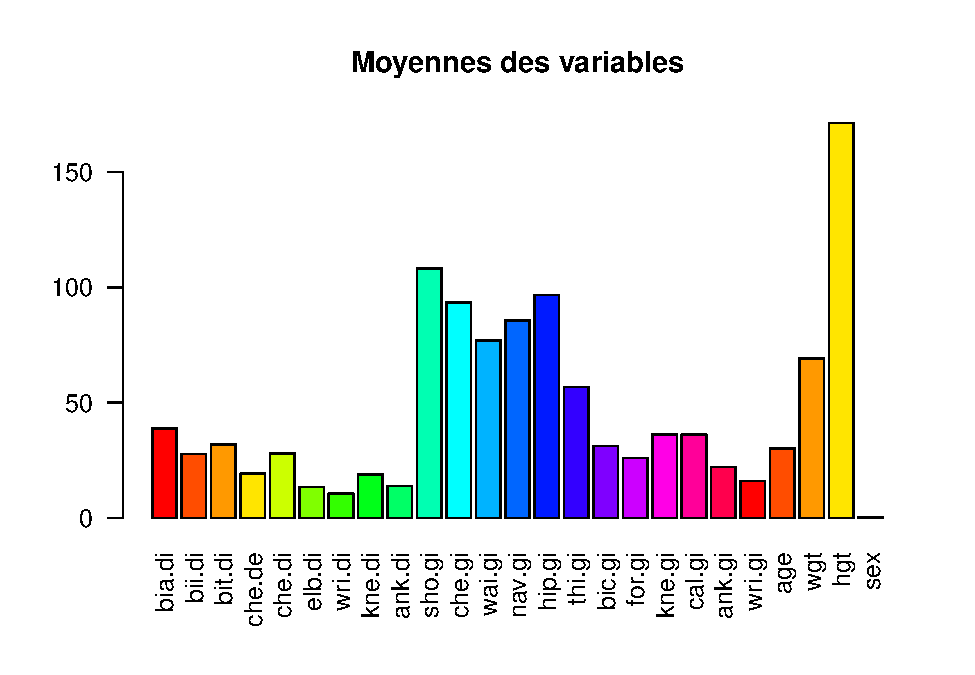
\includegraphics[width=0.33\linewidth]{Template_files/figure-latex/unnamed-chunk-2-1} \end{center}

On voit sur ce barplot que les moyennes ne sont pas toutes comparables.
Le genre (\emph{sex}) étant une variable binaire (et donc aussi
discrète), sa moyenne sera toujours bornée entre zéro et un, alors que
pour les autres variables, qui sont des mesures naturelles, ca n'est pas
le cas. De plus, les unités de mesure de distance (cm) et de poids (kg)
ne sont pas non plus directement comparables. Néanmoins, on remarque
déjà de fortes similarités de moyennes entre certains groupe de zones
anatomiques (ex: les 9 premières, les 5 suivantes et 7 prochaines).

\begin{center}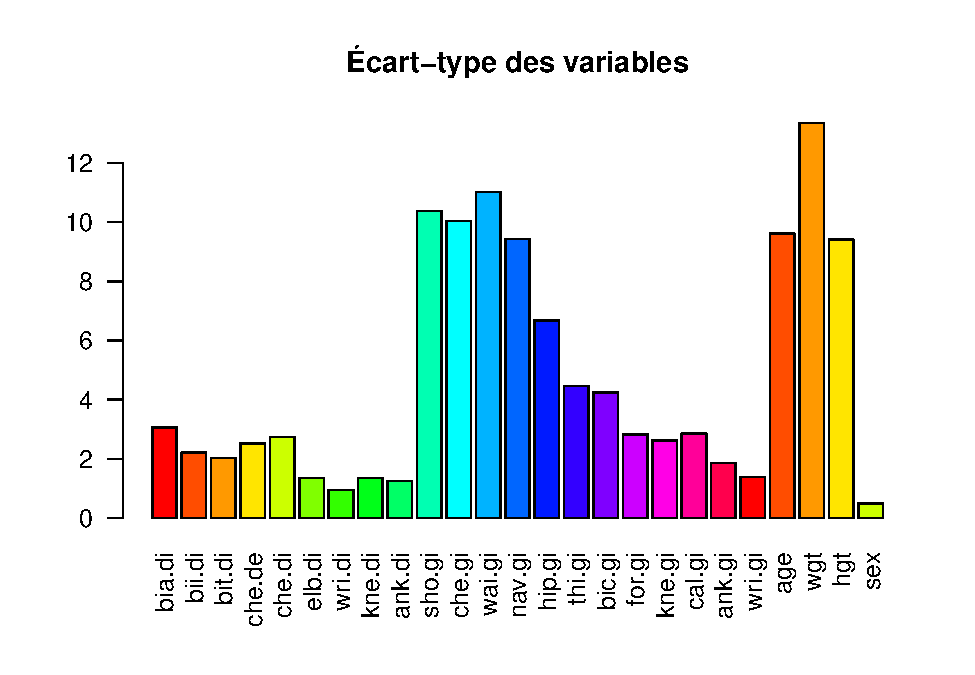
\includegraphics[width=0.33\linewidth]{Template_files/figure-latex/unnamed-chunk-3-1} \end{center}

Ici, on peut observer la moyennes des mesures de diamètre et des mesures
de circonférence de chaque individu. Cela ne nous apporte pas grand
chose à première vue, mais il suffit déjà de prendre l'information du
sexe pour remarquer une différence : les 247 premières moyennes sont des
hommes, et les 260 dernières sont des femmes. On peut donc déjà supposer
qu'une ou plusieurs de ces mesures sont correlées à la variable
catégoricielle du genre.

\begin{center}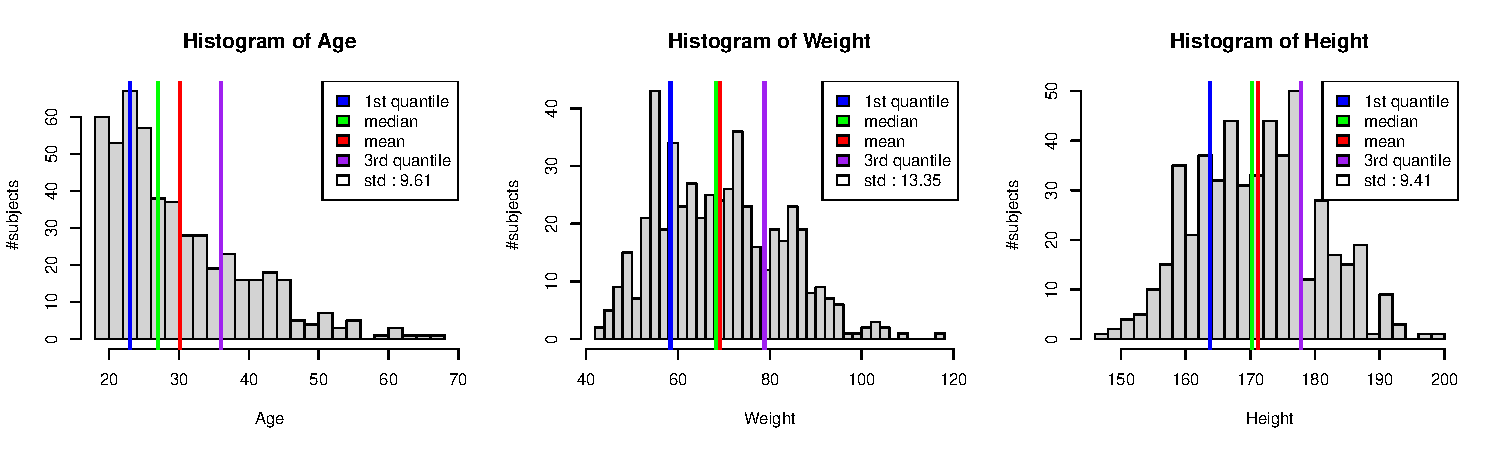
\includegraphics[width=0.33\linewidth]{Template_files/figure-latex/unnamed-chunk-4-1} \end{center}

On remarque que les 9 premières mesures anatomiques n'ont que très peu
de dispersion autour de leur moyenne, comparé aux 5 suivantes. De
nouveau, celles de l'âge, du poids, du sexe et de la taille ne sont pas
encore criticable pour les même raisons déjà évoquées ci-dessus.

\hypertarget{variable-catuxe9goricielle-sex-0-fuxe9minin-1-masculin}{%
\subsection{\texorpdfstring{Variable catégoricielle : \emph{sex} (0 :
Féminin, 1 :
Masculin)}{Variable catégoricielle : sex (0 : Féminin, 1 : Masculin)}}\label{variable-catuxe9goricielle-sex-0-fuxe9minin-1-masculin}}

Cette variable est binaire et discrète. Elle servira à la classification
plus tard dans le rapport. Le nombre d'hommes et de femmes étudiés est
assez équilibré et élevé (247 H - 260 F).

\hypertarget{distribution-des-variables-de-nature-diffuxe9rentes-uxe2ge-taille-et-poids}{%
\subsection{Distribution des variables de nature différentes (âge,
taille et
poids)}\label{distribution-des-variables-de-nature-diffuxe9rentes-uxe2ge-taille-et-poids}}

\begin{center}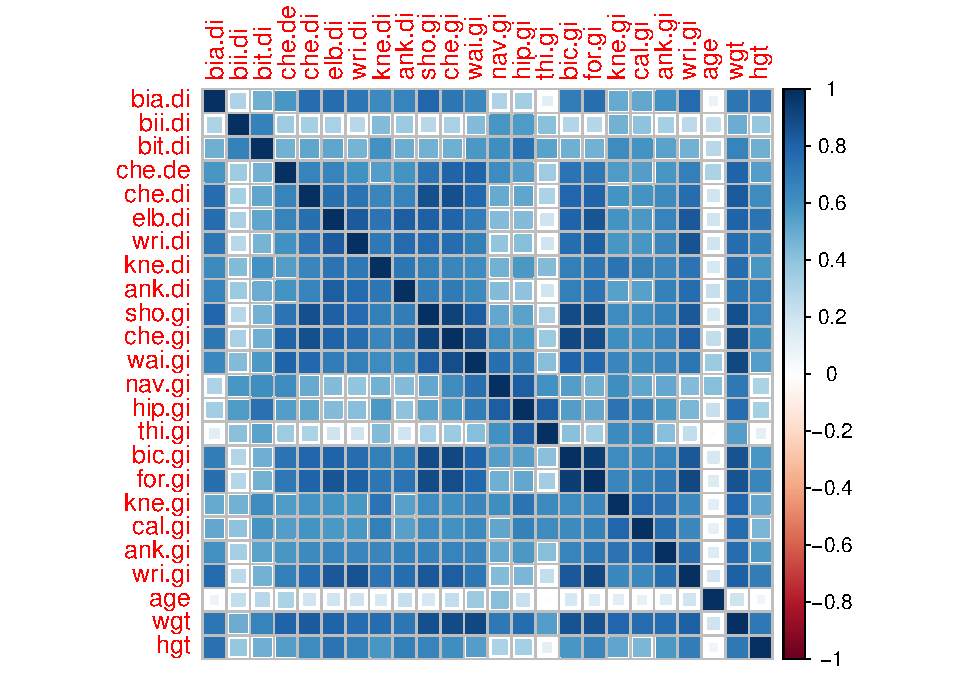
\includegraphics{Template_files/figure-latex/unnamed-chunk-5-1} \end{center}

Ici, nous nous intéressons aux variables autres que les mesures
anatomiques.

On voit sur le premier graphe que la population est assez jeune (30 ans
en moyenne) et que seulement 25\% des individus ont plus de 36 ans,
tandis que 50\% des individus ont moins de 27 ans.

Le second graphe présente presque les mêmes types de quantile et
médiane/moyenne que pourrait le faire une Gaussienne. En effet, la
moyenne et la médiane sont presque identiques, et les 1er et 2eme
quantiles sont équidistants de la moyenne. On note qu'il y'a très peu de
personnes au-dessus de 96 kg, dont un sortant vraiment du lot (116 kg).

La distribution de la taille ressemble encore plus à une Gaussienne que
celle du poids, avec une moyenne à 1m70 et un écart-type de 9.41 cm,
tout genre confondu.

\hypertarget{correlation-entre-les-variables-corrplot}{%
\subsection{Correlation entre les variables :
corrplot}\label{correlation-entre-les-variables-corrplot}}

\begin{center}\includegraphics[width=0.5\linewidth]{Template_files/figure-latex/unnamed-chunk-6-1} \end{center}

Ce plot des corrélation nous indique malheureusement déjà que nous ne
pourrons pas utiliser les mesures anatomiques pour déterminer \emph{age}
(de manière linéaire, car on étudie la corrélation). Étant donné qu'en
plus de ça, la distribution de l'âge n'est pas très représentative de la
population, nous allons donc l'enlever de la base de données. Si on
voulait s'acharner, on pourrait vérifier l'information mutuelle entre la
variable âge et toute les autres, afin de détecter une potentielle
relation non-linéaire.

Remarque supplémentaire : Au vu de ce plot, les variables :
\emph{bii.di}, \emph{thi.gi} seront peu intéressantes.

\hypertarget{analyse-en-composantes-principales}{%
\section{Analyse en composantes
principales}\label{analyse-en-composantes-principales}}

Si on regarde la quantité d'information respectivement apportée par
chaque axe dans le tableau ci-dessous, on peut s'en servir pour choisir
les composantes principales les plus pertinentes.

\begin{center}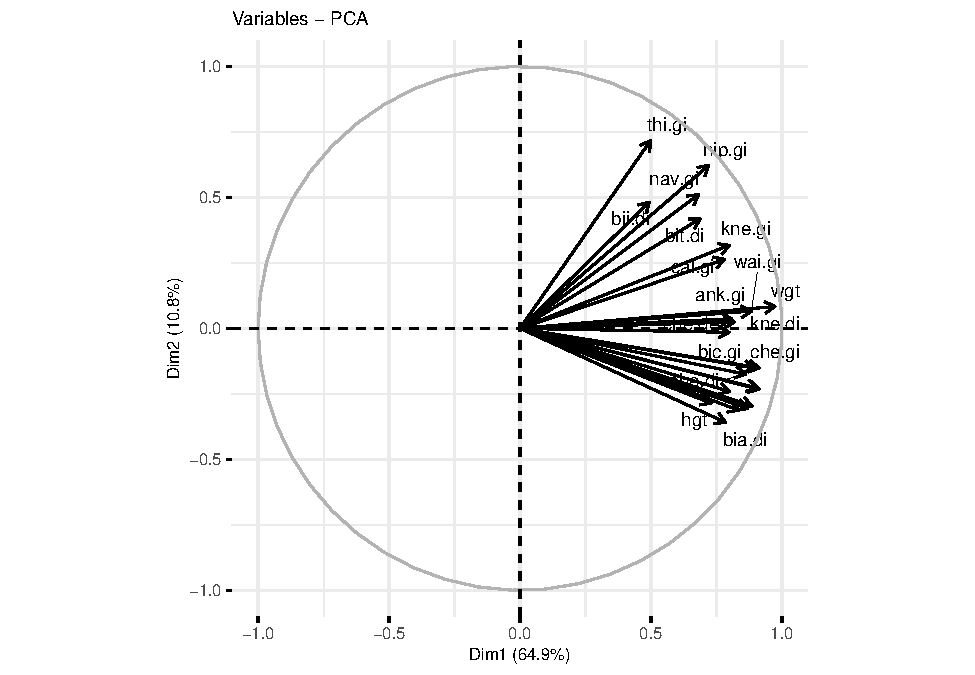
\includegraphics[width=0.33\linewidth]{Template_files/figure-latex/unnamed-chunk-9-1} \end{center}

La « règle du coude » nous encourage à ne retenir que les 2 premiers
axes qui portent environs 73\% de l'information.

La règle de Kaiser nous inciterait à retenir deux axes supplémentaires
(pour un gain de 10\% d'informations), mais un travail beaucoup plus
conséquent.

Nous allons donc retenir les deux premières uniquement.

\begin{center}\includegraphics[width=0.5\linewidth]{Template_files/figure-latex/unnamed-chunk-10-1} \end{center}

\begin{center}\includegraphics[width=0.5\linewidth]{Template_files/figure-latex/unnamed-chunk-10-2} \end{center}

Le cercle des corrélations (et le barplot vert) montre qu'un grand
nombre de variables sont plutôt bien représentées car elles sont très
proche du cercle, leur qualité de représentation (cos2) est toujours
supérieure à 0.5. La seule à être mal représentée est \emph{age} (cos2 =
0.091), d'ou ses mauvais scores de corrélation avec les autres variables
lors du corrplot. Toutes les corrélations sont positives.

Lors du corrplot, nous avions remarqué que les scores de corrélation
bii.di et thi.gi étaient également mauvais. C'est confirmé ici, car on
voit qu'ils sont presque perpendiculaires à la majorité des autres
variables, plus proches de l'axe 1.

\begin{center}\includegraphics[width=0.5\linewidth]{Template_files/figure-latex/unnamed-chunk-11-1} \end{center}

En mappant la variable catégoritielle \emph{sex} sur le graphe des
individus, on peut voir qu'il sont distinctement séparés (hormis
quelques outliers) sur les axes 1 et 2. L'information du sexe se trouve
donc aussi dans d'autre variables, et le fait de n'avoir gardé que 73\%
de l'information en sélectionnant que les deux premières composantes ne
nous a pas fait perdre cette information.

\hypertarget{clustering}{%
\section{Clustering}\label{clustering}}

\begin{verbatim}
Too few points to calculate an ellipse
Too few points to calculate an ellipse
\end{verbatim}

\begin{center}\includegraphics[width=0.5\linewidth]{Template_files/figure-latex/unnamed-chunk-12-1} \end{center}

\hypertarget{analyse-des-correspondances}{%
\section{Analyse des
correspondances}\label{analyse-des-correspondances}}

Comme vu en TP, grâce aux relations quasi-barycentriques, nous pouvons
représenter sur le même graphique à la fois les coordonnées factorielles
des lignes et des colonnes et leur proximité/éloignement a donc une
interprétation intrinsèque en termes de liens. Afin de faciliter cette
interprétation, on représente généralement les coordonnées de l'ACFS sur
le premier plan factoriel. Le graphe de la quantité d'information
relative à chaque axe principal ci-dessous nous indique que c'est
acceptable, même si prendre également le 3e axe est tentant.

\begin{center}\includegraphics[width=0.33\linewidth]{Template_files/figure-latex/unnamed-chunk-13-1} \end{center}

Si maintenant, on affiche le graphe des individus et des variables, on
ne sait pas interprêter grand chose, car les individus sont trop
nombreux, hormis que le mappage du genre est logiquement conservé avec
l'AFC.

Néanmoins, si on mappe la valeur du BMI de chaque individu sur chacun
des points du graphe des individus, on peut voir une tendance très nette
(S-E vers N-O). Cette tendance se justifie par la position des variables
\emph{wgt} et \emph{hgt} dans le graphe des variables, malgré que la
formule du BMI ne soit pas linéaire. La taille (\emph{hgt}) a une
influence négative sur le BMI, alors que le poids (\emph{wgt}) a une
influence positive.

\includegraphics[width=0.32\linewidth]{Template_files/figure-latex/unnamed-chunk-14-1}
\includegraphics[width=0.32\linewidth]{Template_files/figure-latex/unnamed-chunk-14-2}
\includegraphics[width=0.32\linewidth]{Template_files/figure-latex/unnamed-chunk-14-3}

\begin{center}\includegraphics[width=0.33\linewidth]{Template_files/figure-latex/unnamed-chunk-15-1} \end{center}

Sur le barplot des Cos2, hip.gi et le poids (\emph{wgt}) sont les mieux
représentés dans le premier plan factoriel. Un peu moins de la moitié
des variables sont sous la barre des 50\%, elles ne sont pas assez
représentées que pour être analysées. La quantité d'individu est trop
vaste que pour afficher le graphe équivalent, mais la qualité de
représentation minimale chez eux est de : 0.013 (individu n°488 : une
femme de 1m62 et 70kg).

\begin{center}\includegraphics[width=0.33\linewidth]{Template_files/figure-latex/unnamed-chunk-16-1} \end{center}

\begin{longtable}[]{@{}
  >{\centering\arraybackslash}p{(\columnwidth - 14\tabcolsep) * \real{0.16}}
  >{\centering\arraybackslash}p{(\columnwidth - 14\tabcolsep) * \real{0.12}}
  >{\centering\arraybackslash}p{(\columnwidth - 14\tabcolsep) * \real{0.12}}
  >{\centering\arraybackslash}p{(\columnwidth - 14\tabcolsep) * \real{0.12}}
  >{\centering\arraybackslash}p{(\columnwidth - 14\tabcolsep) * \real{0.12}}
  >{\centering\arraybackslash}p{(\columnwidth - 14\tabcolsep) * \real{0.12}}
  >{\centering\arraybackslash}p{(\columnwidth - 14\tabcolsep) * \real{0.12}}
  >{\centering\arraybackslash}p{(\columnwidth - 14\tabcolsep) * \real{0.12}}@{}}
\caption{Table continues below}\tabularnewline
\toprule
\begin{minipage}[b]{\linewidth}\centering
~
\end{minipage} & \begin{minipage}[b]{\linewidth}\centering
bia.di
\end{minipage} & \begin{minipage}[b]{\linewidth}\centering
bii.di
\end{minipage} & \begin{minipage}[b]{\linewidth}\centering
bit.di
\end{minipage} & \begin{minipage}[b]{\linewidth}\centering
che.de
\end{minipage} & \begin{minipage}[b]{\linewidth}\centering
che.di
\end{minipage} & \begin{minipage}[b]{\linewidth}\centering
elb.di
\end{minipage} & \begin{minipage}[b]{\linewidth}\centering
wri.di
\end{minipage} \\
\midrule
\endfirsthead
\toprule
\begin{minipage}[b]{\linewidth}\centering
~
\end{minipage} & \begin{minipage}[b]{\linewidth}\centering
bia.di
\end{minipage} & \begin{minipage}[b]{\linewidth}\centering
bii.di
\end{minipage} & \begin{minipage}[b]{\linewidth}\centering
bit.di
\end{minipage} & \begin{minipage}[b]{\linewidth}\centering
che.de
\end{minipage} & \begin{minipage}[b]{\linewidth}\centering
che.di
\end{minipage} & \begin{minipage}[b]{\linewidth}\centering
elb.di
\end{minipage} & \begin{minipage}[b]{\linewidth}\centering
wri.di
\end{minipage} \\
\midrule
\endhead
\textbf{Dim 1} & 0.574 & 3.493 & 3.092 & 1.151 & 0.138 & 0.028 &
0.014 \\
\textbf{Dim 2} & 5.774 & 1.327 & 0.392 & 0.008 & 1.499 & 1.644 &
1.056 \\
\bottomrule
\end{longtable}

\begin{longtable}[]{@{}
  >{\centering\arraybackslash}p{(\columnwidth - 14\tabcolsep) * \real{0.16}}
  >{\centering\arraybackslash}p{(\columnwidth - 14\tabcolsep) * \real{0.12}}
  >{\centering\arraybackslash}p{(\columnwidth - 14\tabcolsep) * \real{0.12}}
  >{\centering\arraybackslash}p{(\columnwidth - 14\tabcolsep) * \real{0.12}}
  >{\centering\arraybackslash}p{(\columnwidth - 14\tabcolsep) * \real{0.12}}
  >{\centering\arraybackslash}p{(\columnwidth - 14\tabcolsep) * \real{0.12}}
  >{\centering\arraybackslash}p{(\columnwidth - 14\tabcolsep) * \real{0.12}}
  >{\centering\arraybackslash}p{(\columnwidth - 14\tabcolsep) * \real{0.12}}@{}}
\caption{Table continues below}\tabularnewline
\toprule
\begin{minipage}[b]{\linewidth}\centering
~
\end{minipage} & \begin{minipage}[b]{\linewidth}\centering
kne.di
\end{minipage} & \begin{minipage}[b]{\linewidth}\centering
ank.di
\end{minipage} & \begin{minipage}[b]{\linewidth}\centering
sho.gi
\end{minipage} & \begin{minipage}[b]{\linewidth}\centering
che.gi
\end{minipage} & \begin{minipage}[b]{\linewidth}\centering
wai.gi
\end{minipage} & \begin{minipage}[b]{\linewidth}\centering
nav.gi
\end{minipage} & \begin{minipage}[b]{\linewidth}\centering
hip.gi
\end{minipage} \\
\midrule
\endfirsthead
\toprule
\begin{minipage}[b]{\linewidth}\centering
~
\end{minipage} & \begin{minipage}[b]{\linewidth}\centering
kne.di
\end{minipage} & \begin{minipage}[b]{\linewidth}\centering
ank.di
\end{minipage} & \begin{minipage}[b]{\linewidth}\centering
sho.gi
\end{minipage} & \begin{minipage}[b]{\linewidth}\centering
che.gi
\end{minipage} & \begin{minipage}[b]{\linewidth}\centering
wai.gi
\end{minipage} & \begin{minipage}[b]{\linewidth}\centering
nav.gi
\end{minipage} & \begin{minipage}[b]{\linewidth}\centering
hip.gi
\end{minipage} \\
\midrule
\endhead
\textbf{Dim 1} & 0.66 & 0.087 & 1.258 & 4.242 & 14.53 & 0.046 & 5.321 \\
\textbf{Dim 2} & 0.21 & 0.891 & 8.207 & 2.161 & 2.816 & 34.18 & 10.47 \\
\bottomrule
\end{longtable}

\begin{longtable}[]{@{}
  >{\centering\arraybackslash}p{(\columnwidth - 14\tabcolsep) * \real{0.16}}
  >{\centering\arraybackslash}p{(\columnwidth - 14\tabcolsep) * \real{0.12}}
  >{\centering\arraybackslash}p{(\columnwidth - 14\tabcolsep) * \real{0.12}}
  >{\centering\arraybackslash}p{(\columnwidth - 14\tabcolsep) * \real{0.12}}
  >{\centering\arraybackslash}p{(\columnwidth - 14\tabcolsep) * \real{0.12}}
  >{\centering\arraybackslash}p{(\columnwidth - 14\tabcolsep) * \real{0.12}}
  >{\centering\arraybackslash}p{(\columnwidth - 14\tabcolsep) * \real{0.12}}
  >{\centering\arraybackslash}p{(\columnwidth - 14\tabcolsep) * \real{0.12}}@{}}
\caption{Table continues below}\tabularnewline
\toprule
\begin{minipage}[b]{\linewidth}\centering
~
\end{minipage} & \begin{minipage}[b]{\linewidth}\centering
thi.gi
\end{minipage} & \begin{minipage}[b]{\linewidth}\centering
bic.gi
\end{minipage} & \begin{minipage}[b]{\linewidth}\centering
for.gi
\end{minipage} & \begin{minipage}[b]{\linewidth}\centering
kne.gi
\end{minipage} & \begin{minipage}[b]{\linewidth}\centering
cal.gi
\end{minipage} & \begin{minipage}[b]{\linewidth}\centering
ank.gi
\end{minipage} & \begin{minipage}[b]{\linewidth}\centering
wri.gi
\end{minipage} \\
\midrule
\endfirsthead
\toprule
\begin{minipage}[b]{\linewidth}\centering
~
\end{minipage} & \begin{minipage}[b]{\linewidth}\centering
thi.gi
\end{minipage} & \begin{minipage}[b]{\linewidth}\centering
bic.gi
\end{minipage} & \begin{minipage}[b]{\linewidth}\centering
for.gi
\end{minipage} & \begin{minipage}[b]{\linewidth}\centering
kne.gi
\end{minipage} & \begin{minipage}[b]{\linewidth}\centering
cal.gi
\end{minipage} & \begin{minipage}[b]{\linewidth}\centering
ank.gi
\end{minipage} & \begin{minipage}[b]{\linewidth}\centering
wri.gi
\end{minipage} \\
\midrule
\endhead
\textbf{Dim 1} & 5.991 & 4.125 & 0.786 & 1.458 & 1.045 & 0.328 &
0.005 \\
\textbf{Dim 2} & 8.841 & 1.288 & 2.251 & 0.241 & 0.084 & 0.107 & 1.49 \\
\bottomrule
\end{longtable}

\begin{longtable}[]{@{}
  >{\centering\arraybackslash}p{(\columnwidth - 4\tabcolsep) * \real{0.17}}
  >{\centering\arraybackslash}p{(\columnwidth - 4\tabcolsep) * \real{0.11}}
  >{\centering\arraybackslash}p{(\columnwidth - 4\tabcolsep) * \real{0.11}}@{}}
\toprule
\begin{minipage}[b]{\linewidth}\centering
~
\end{minipage} & \begin{minipage}[b]{\linewidth}\centering
wgt
\end{minipage} & \begin{minipage}[b]{\linewidth}\centering
hgt
\end{minipage} \\
\midrule
\endhead
\textbf{Dim 1} & 37.14 & 14.48 \\
\textbf{Dim 2} & 1.425 & 13.63 \\
\bottomrule
\end{longtable}

Les variables qui contribuent le plus au premier plan factoriel sont les
plus importantes pour expliquer la variabilité du set de données. Les
variables qui ne contribuent pas beaucoup à une dimension ou qui
contribuent aux dernières dimensions sont moins importantes. Sur le
premier axe, la différenciation des individus se fait surtout par le
poids \emph{wgt}, la taille \emph{hgt} et \emph{wai.gi}, tandis que sur
le deuxième axe, elle se fais principalement par la variable
\emph{nav.gi}.

\hypertarget{conclusions}{%
\section{Conclusions}\label{conclusions}}

\hypertarget{annexes}{%
\section{Annexes}\label{annexes}}

\hypertarget{duxe9finition-des-donnuxe9es}{%
\subsection{Définition des données}\label{duxe9finition-des-donnuxe9es}}

\begin{itemize}
\tightlist
\item
  \emph{bia.di} : Un vecteur numérique, le diamètre biacromial du sujet
  en centimètres.
\item
  \emph{bii.di} : Un vecteur numérique, le diamètre biiliaque du sujet
  (largeur pelvienne) en centimètres.
\item
  \emph{bit.di} : Un vecteur numérique, le diamètre bitrochantérien du
  sujet en centimètres.
\end{itemize}

\begin{figure}
\centering
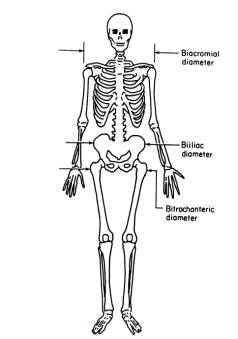
\includegraphics{johnson_figure2.jpg}
\caption{Biacromial, Biiliac, and Bitrochanteric Diameters.}
\end{figure}

\begin{itemize}
\tightlist
\item
  \emph{che.de} : un vecteur numérique, la profondeur de la poitrine du
  sujet en centimètres, mesurée entre la colonne vertébrale et le
  sternum au niveau du mamelon, à mi-expiration.
\item
  \emph{che.di} : Un vecteur numérique, le diamètre thoracique du sujet
  en centimètres, mesuré au niveau du mamelon, à mi-expiration.
\item
  \emph{elb.di} : Un vecteur numérique, le diamètre du coude du sujet en
  centimètres, mesuré comme la somme de deux coudes.
\item
  \emph{wri.di} : Un vecteur numérique, le diamètre du poignet du sujet
  en centimètres, mesuré comme la somme de deux poignets.
\item
  \emph{kne.di} : Un vecteur numérique, le diamètre du genou du sujet en
  centimètres, mesuré comme la somme de deux genoux.
\item
  \emph{ank.di} : Un vecteur numérique, le diamètre de la cheville du
  sujet en centimètres, mesuré comme la somme de deux chevilles.
\item
  \emph{sho.gi} : un vecteur numérique, la circonférence de l'épaule du
  sujet en centimètres, mesurée sur les muscles deltoïdes.
\item
  \emph{che.gi} : Un vecteur numérique, le tour de poitrine du sujet en
  centimètres, mesuré à la ligne du mamelon chez les hommes et juste
  au-dessus du tissu mammaire chez les femmes, à mi-expiration.
\item
  \emph{wai.gi} : un vecteur numérique, le tour de taille du sujet en
  centimètres, mesuré à la partie la plus étroite du torse sous la cage
  thoracique comme moyenne de la position contractée et détendue.
\item
  \emph{nav.gi} : un vecteur numérique, la circonférence du nombril
  (abdominale) du sujet en centimètres, mesurée au niveau de l'ombilic
  et de la crête iliaque en utilisant la crête iliaque comme point de
  repère.
\item
  \emph{hip.gi} : Un vecteur numérique, la circonférence de la hanche du
  sujet en centimètres, mesurée au niveau du diamètre bitrochantérien.
\item
  \emph{thi.gi} : Un vecteur numérique, la circonférence de la cuisse du
  sujet en centimètres, mesurée sous le pli fessier comme la moyenne des
  circonférences droite et gauche.
\item
  \emph{bic.gi} : Un vecteur numérique, la circonférence du biceps du
  sujet en centimètres, mesurée lorsqu'elle est fléchie comme la moyenne
  des circonférences droite et gauche.
\item
  \emph{for.gi} : Un vecteur numérique, la circonférence de l'avant-bras
  du sujet en centimètres, mesurée lorsqu'elle est étendue, paume vers
  le haut comme moyenne des circonférences droite et gauche.
\item
  \emph{kne.gi} : Un vecteur numérique, le diamètre du genou du sujet en
  centimètres, mesuré comme la somme de deux genoux.
\item
  \emph{cal.gi} : Un vecteur numérique, la circonférence maximale du
  mollet du sujet en centimètres, mesurée comme la moyenne des
  circonférences droite et gauche.
\item
  \emph{ank.gi} : un vecteur numérique, la circonférence minimale de la
  cheville du sujet en centimètres, mesurée comme la moyenne des
  circonférences droite et gauche.
\item
  \emph{wri.gi} : un vecteur numérique, la circonférence minimale du
  poignet du sujet en centimètres, mesurée comme la moyenne des
  circonférences droite et gauche.
\item
  \emph{age} : Un vecteur numérique, l'âge du sujet en années.
\item
  \emph{wgt} : Un vecteur numérique, le poids du sujet en kilogrammes.
\item
  \emph{hgt} : Un vecteur numérique, la taille du sujet en centimètres.
\item
  \emph{sex} : Un vecteur catégoriel, 1 si le sujet est un homme, 0 si
  une femme.
\end{itemize}

\end{document}
